%%
%% This is file `sample-manuscript.tex',
%% generated with the docstrip utility.
%%
%% The original source files were:
%%
%% samples.dtx  (with options: `all,proceedings,bibtex,manuscript')
%% 
%% IMPORTANT NOTICE:
%% 
%% For the copyright see the source file.
%% 
%% Any modified versions of this file must be renamed
%% with new filenames distinct from sample-manuscript.tex.
%% 
%% For distribution of the original source see the terms
%% for copying and modification in the file samples.dtx.
%% 
%% This generated file may be distributed as long as the
%% original source files, as listed above, are part of the
%% same distribution. (The sources need not necessarily be
%% in the same archive or directory.)
%%
%%
%% Commands for TeXCount
%TC:macro \cite [option:text,text]
%TC:macro \citep [option:text,text]
%TC:macro \citet [option:text,text]
%TC:envir table 0 1
%TC:envir table* 0 1
%TC:envir tabular [ignore] word
%TC:envir displaymath 0 word
%TC:envir math 0 word
%TC:envir comment 0 0
%%
%% The first command in your LaTeX source must be the \documentclass
%% command.
%%
%% For submission and review of your manuscript please change the
%% command to \documentclass[manuscript, screen, review]{acmart}.
%%
%% When submitting camera ready or to TAPS, please change the command
%% to \documentclass[sigconf]{acmart} or whichever template is required
%% for your publication.
%%
%%
\documentclass[manuscript]{acmart}
%%
%% \BibTeX command to typeset BibTeX logo in the docs
\AtBeginDocument{%
  \providecommand\BibTeX{{%
    Bib\TeX}}}

%% Rights management information.  This information is sent to you
%% when you complete the rights form.  These commands have SAMPLE
%% values in them; it is your responsibility as an author to replace
%% the commands and values with those provided to you when you
%% complete the rights form.\


%%
%% Submission ID.
%% Use this when submitting an article to a sponsored event. You'll
%% receive a unique submission ID from the organizers
%% of the event, and this ID should be used as the parameter to this command.
%%\acmSubmissionID{123-A56-BU3}

%%
%% For managing citations, it is recommended to use bibliography
%% files in BibTeX format.
%%
%% You can then either use BibTeX with the ACM-Reference-Format style,
%% or BibLaTeX with the acmnumeric or acmauthoryear sytles, that include
%% support for advanced citation of software artefact from the
%% biblatex-software package, also separately available on CTAN.
%%
%% Look at the sample-*-biblatex.tex files for templates showcasing
%% the biblatex styles.
%%
%%
%% The majority of ACM publications use numbered citations and
%% references.  The command \citestyle{authoryear} switches to the
%% "author year" style.
%%
%% If you are preparing content for an event
%% sponsored by ACM SIGGRAPH, you must use the "author year" style of
%% citations and references.
%% Uncommenting
%% the next command will enable that style.
%%\citestyle{acmauthoryear}


%%
%% end of the preamble, start of the body of the document source.
\begin{document}

%%
%% The "title" command has an optional parameter,
%% allowing the author to define a "short title" to be used in page headers.
\title{Reimagining Transit Networks: A Data-Driven, Algorithmic Approach for the Washington DC Region}

%%
%% The "author" command and its associated commands are used to define
%% the authors and their affiliations.
%% Of note is the shared affiliation of the first two authors, and the
%% "authornote" and "authornotemark" commands
%% used to denote shared contribution to the research.
\author{Spencer Jenkins}


%%
%% By default, the full list of authors will be used in the page
%% headers. Often, this list is too long, and will overlap
%% other information printed in the page headers. This command allows
%% the author to define a more concise list
%% of authors' names for this purpose.
\renewcommand{\shortauthors}{Trovato et al.}

%%
%% The abstract is a short summary of the work to be presented in the
%% article.
\begin{abstract}
This paper presents a computational framework for the design of a reimagined rapid transit network for the Washington, DC metropolitan area. Motivated by the historical context and limitations of the existing WMATA system, my approach leverages geospatial analysis, graph algorithms, and data visualization to generate and evaluate alternative transit networks. The project consists of a transit network development pipeline, and a program to visualize and evaluate the generated networks. I describe the data sources, algorithms, and evaluation metrics used, and discuss the implications of my results for urban mobility and equity.
\end{abstract}

%%
%% This command processes the author and affiliation and title
%% information and builds the first part of the formatted document.
\maketitle



\section{Introduction}

This project was completed for CMSC 725: Geospatial Algorithms and Data, taught by Professor Hanan Samet. 

Public transportation is a critical component of urban infrastructure, associated with increased economic productivity~\cite{lit:us_transit_policy}, social equity~\cite{lit:equity}, and environmental sustainability~\cite{lit:us_transit_policy} in metropolitan areas. Washington, DC, and its surrounding areas in Maryland and Virginia, comprise the second-largest rapid transit network in the United States by daily ridership~\cite{lit:wmata_stats}. The network consists of six heavy rail lines spanning 208 kilometers and connecting 98 stations, operated by the Washington Metropolitan Area Transit Authority (WMATA)~\cite{lit:wmata_stats}. In 2019, the Washington Metro provided over 160 million trips per year, including work commutes, tourism, and other purposes~\cite{lit:wmata_stats}.

A primary objective in designing public transit networks in the U.S. is to reduce car dependency~\cite{lit:us_transit_policy}. However, the Washington Metro has struggled to achieve this, with only about 14\% of commuters in the region using transit~\cite{lit:commute_stats}. Comparable metropolitan areas such as Toronto report higher transit commute shares, while many European and Latin American cities also have significantly higher shares~\cite{lit:toronto}. These statistics are typically limited to work commutes, as data for other trip types is less available~\cite{lit:commute_stats}.

The limited success of the Washington Metro in attracting ridership is largely attributable to the priorities at the time of its planning~\cite{lit:wmata_history}. Unlike older East Coast cities with legacy rail systems, the Metro was conceived in the 1950s, an era of expanding car infrastructure and urban expressways. The Metro was designed as a compromise, connecting car commuters to the city center, with expansions primarily serving suburban areas~\cite{lit:wmata_history}. As a result, the network remains largely radial and focused on suburban commuters.

This project leverages core concepts from CMSC 725, including spatial data structures (such as quadtrees and B-trees), proximity graphs, and efficient spatial querying, to address the challenges of transit network design. The methodology integrates geospatial analysis, graph algorithms, and data-driven optimization to generate and evaluate alternative transit networks for the Washington, DC region. By applying techniques from the course, such as kernel density estimation for spatial demand modeling and the use of Gabriel graphs for candidate network construction, the project demonstrates the power of computational geometry and geospatial algorithms in solving real-world urban problems.

This design ethos limits practical use. The network makes suburb-to-suburb and circumferential travel difficult, often requiring passengers to travel into the city center and transfer, even for short cross-town trips~\cite{lit:wmata_stats}. High-density neighborhoods such as Georgetown and marginalized areas like Anacostia have been historically underserved due to political, financial, and social factors~\cite{lit:equity}. Despite significant investment, the Metro has not achieved a substantial reduction in vehicle miles traveled (VMT) or car dependency~\cite{lit:env}. The static nature of the network has also hindered adaptation to shifting population centers and job clusters.

The persistent gaps in the current network's ability to connect high-density and underserved regions further motivate a new approach. For example, the lack of direct connections between major suburban job centers or marginalized neighborhoods limits economic opportunity and social inclusion~\cite{lit:equity}. Existing evaluation frameworks may overlook these gaps, focusing on aggregate metrics that mask disparities in access and service quality. 

To address these challenges, this study combines computational and geospatial techniques to generate, evaluate, and visualize alternative transit networks for the Washington, DC region. 

% --- Table: Counties and FIPS codes ---

% Table 1: Counties and County-Equivalents Considered

\begin{table}[h]
\caption{Counties and County-Equivalents in the Study Area}
\label{tab:counties}
\begin{tabular}{lccc}
\toprule
County/Equivalent & 2020 Population & Density (per km$^2$) & FIPS Code \\
\midrule
Prince George's & [value] & [value] & [value] \\
Montgomery & [value] & [value] & [value] \\
District of Columbia & [value] & [value] & [value] \\
Arlington County & [value] & [value] & [value] \\
Alexandria City & [value] & [value] & [value] \\
Falls Church City & [value] & [value] & [value] \\
Fairfax County & [value] & [value] & [value] \\
Fairfax City & [value] & [value] & [value] \\
Loudoun County & [value] & [value] & [value] \\
\bottomrule
\end{tabular}
\end{table}

% --- Table: Data Sources ---

\begin{table}[h]
\caption{Key Data Sources Used in the Study}
\label{tab:datasources}
\begin{tabular}{ll}
\toprule
Source & Description \\
\midrule
US Census Bureau & Census block population, shapefiles \\
Open Data DC/MD/VA & Points of interest, transit stops, land use \\
Arlington County & Neighborhood boundaries \\
State of Maryland & Neighborhood boundaries \\
District of Columbia & Neighborhood centroids \\
WMATA & Existing transit network \\
\bottomrule
\end{tabular}
\end{table}

% --- Figure: KDE Map ---

\begin{figure}[h]
    \centering
    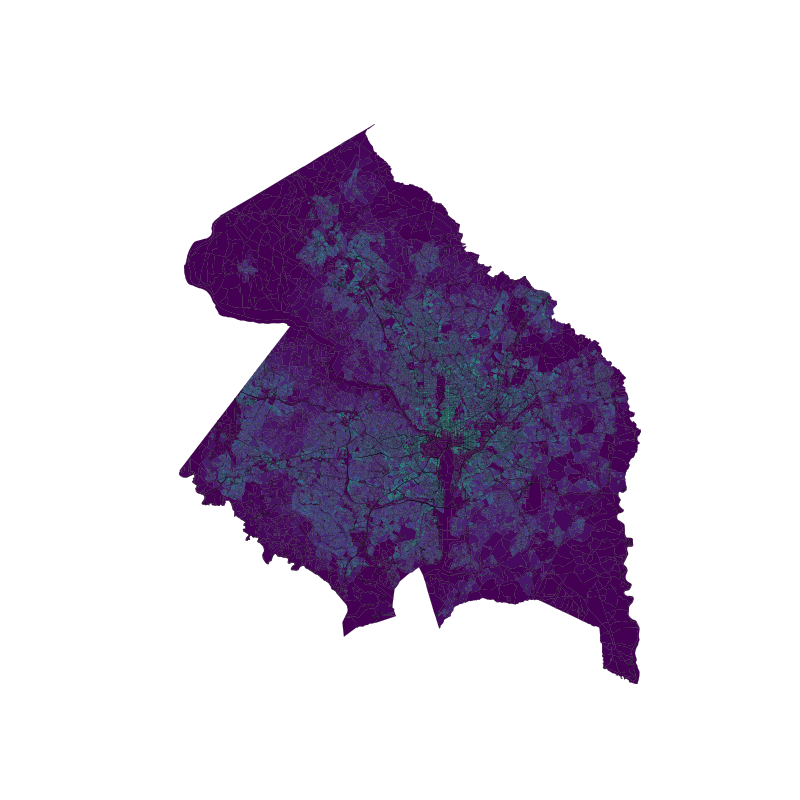
\includegraphics[width=0.7\textwidth]{img/transit_potential.png}
    \caption{Kernel density estimation (KDE) map of transit potential in the Washington, DC region.}
    \label{fig:kde}
\end{figure}

% --- Figure: Network Map Example ---

\begin{figure}[h]
    \centering
    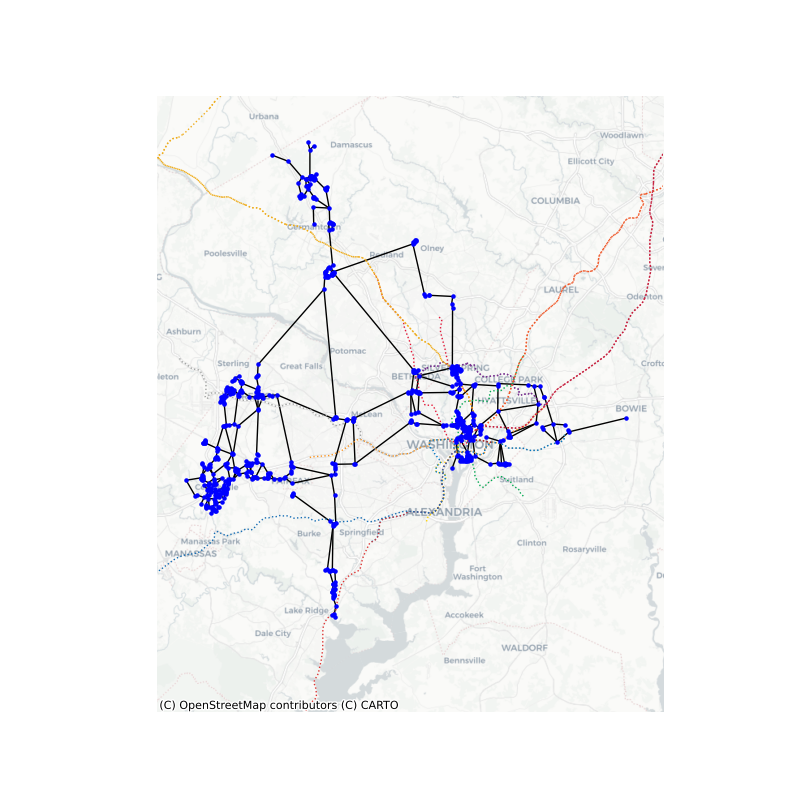
\includegraphics[width=0.7\textwidth]{img/network_map.png}
    \caption{Example of a generated candidate network overlaid on the metropolitan area.}
    \label{fig:networkmap}
\end{figure}

% --- Figure: Schematic Map Example ---

\begin{figure}[h]
    \centering
    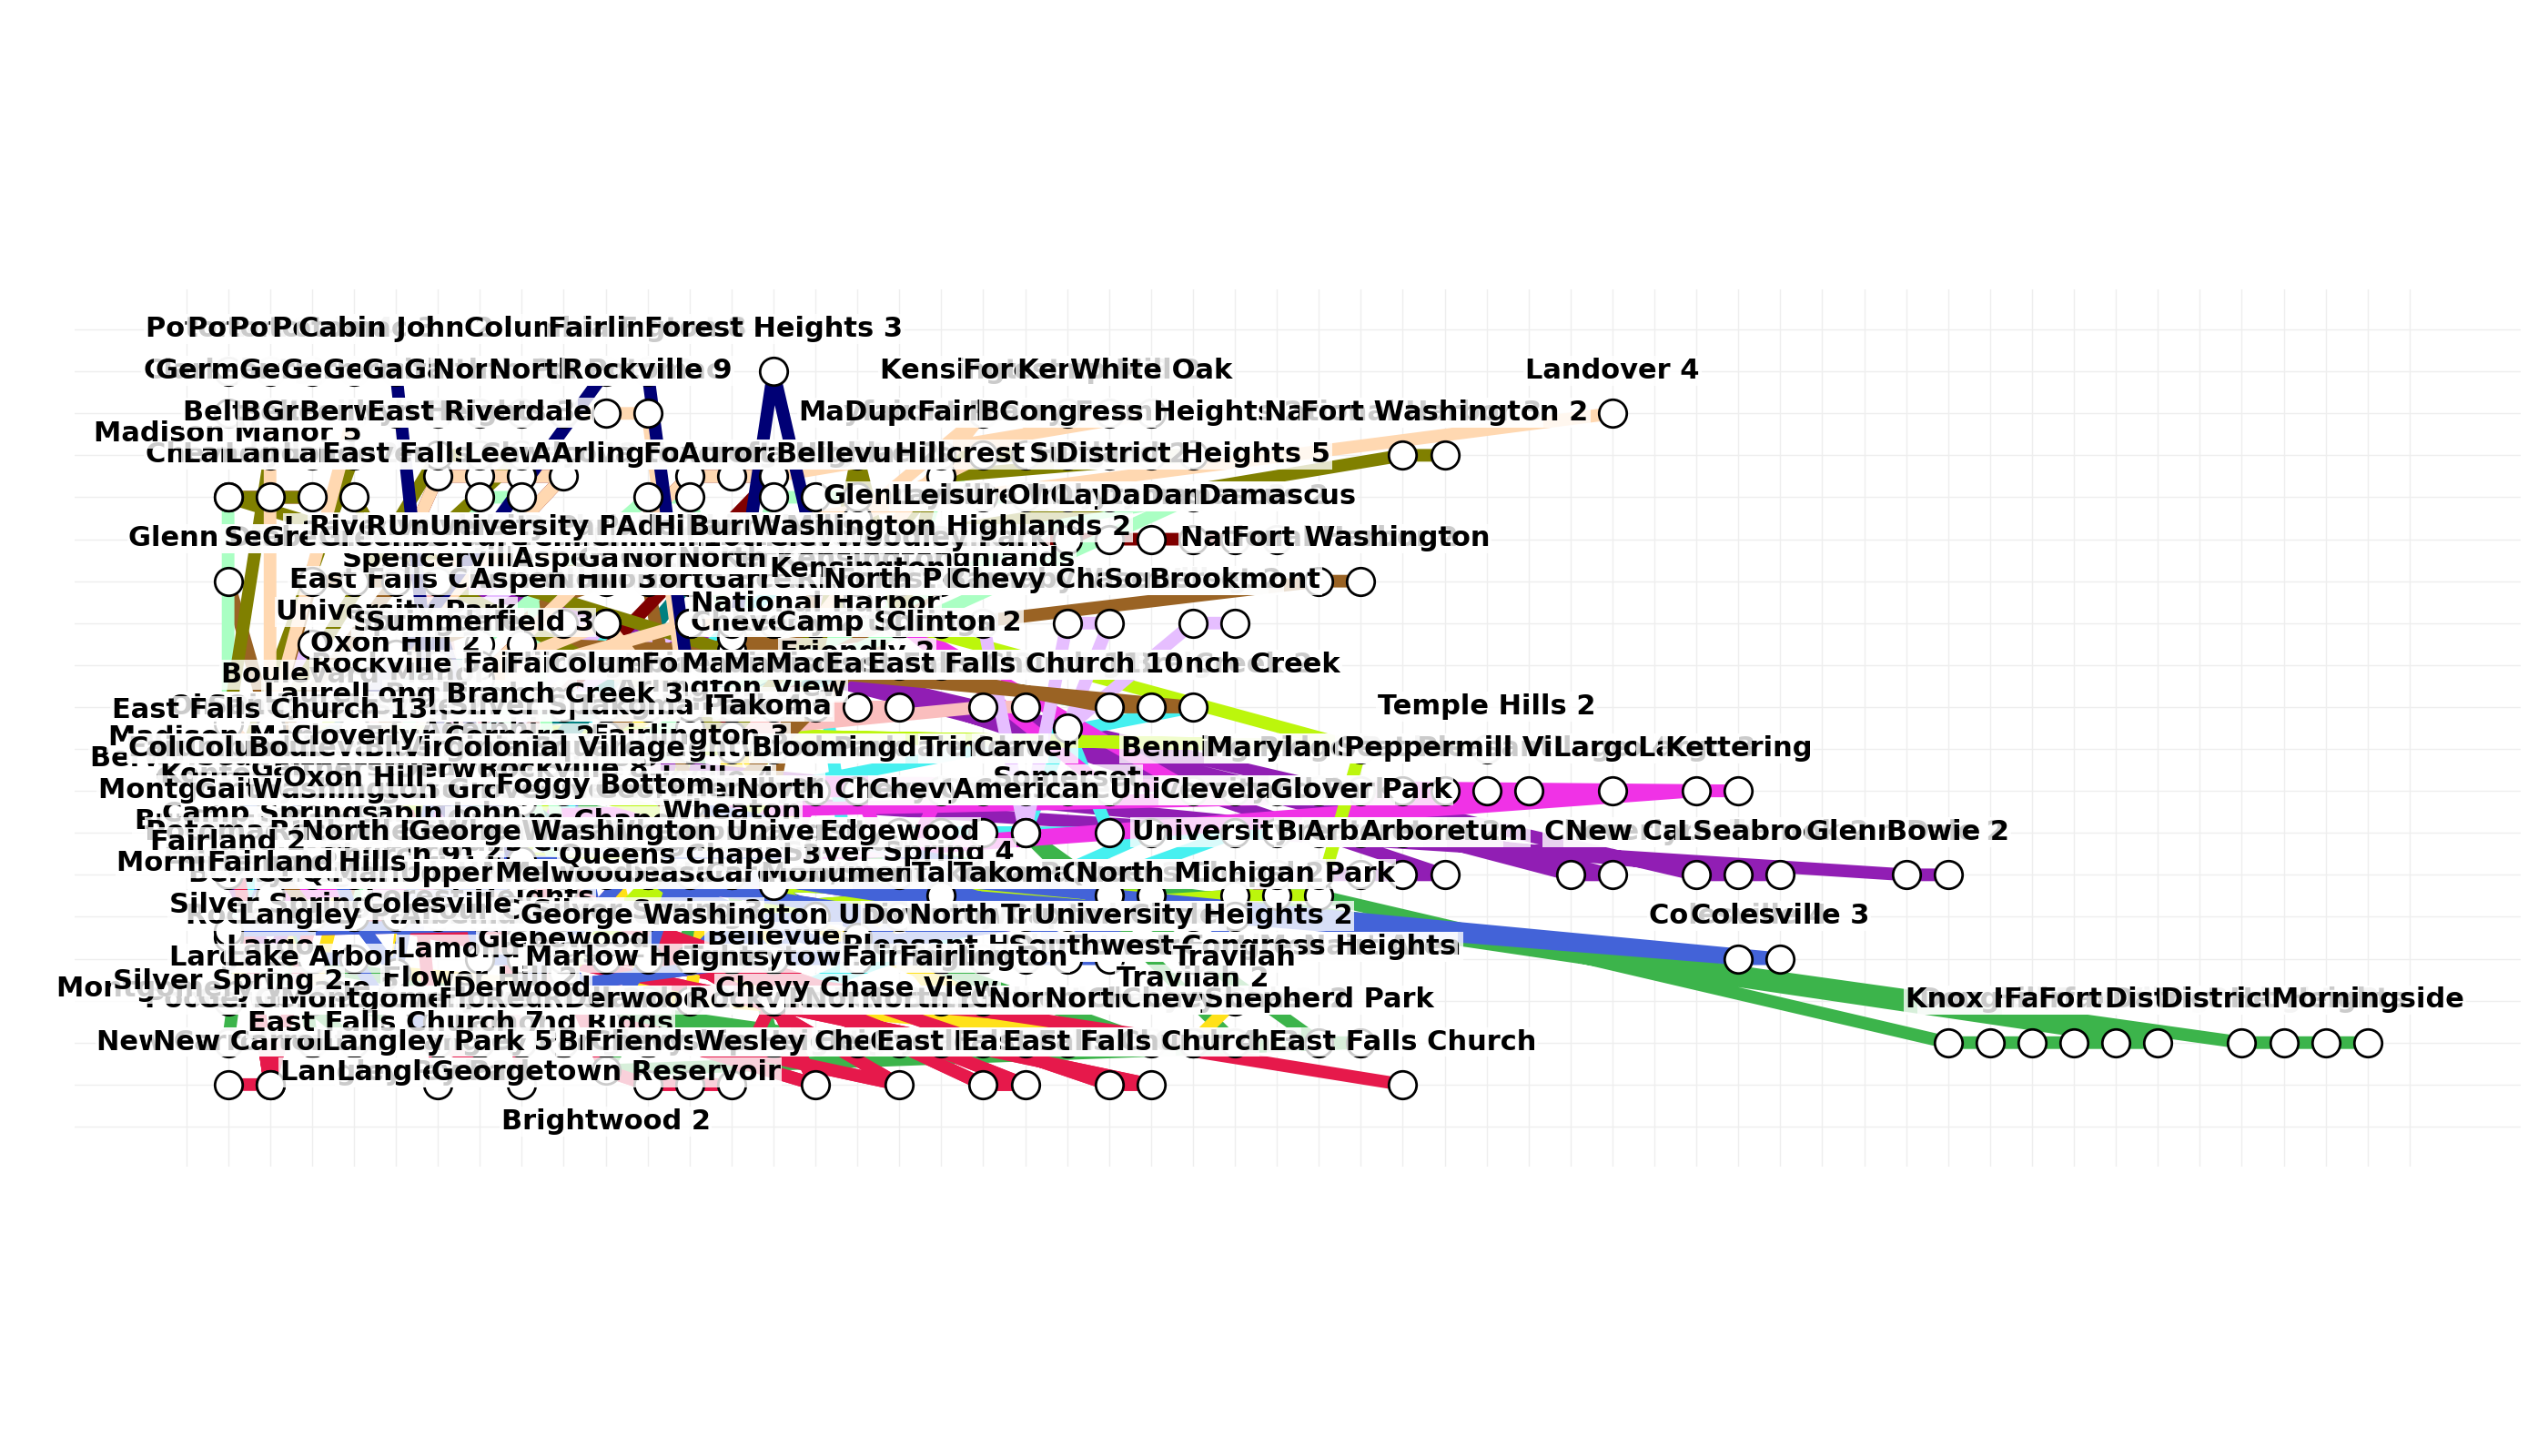
\includegraphics[width=0.7\textwidth]{img/lines_genetic.png}
    \caption{Schematic map of a generated network using the genetic algorithm.}
    \label{fig:schematic}
\end{figure}

\section{Network Design}

In this section, the network design process is detailed, including data collection, transformation, metric construction, network generation constraints, and the definition of the transit network search space. The network is built within this search space according to the scoring metrics and constraints, followed by post-processing.

\subsection{Data Sources and Transformation}
The first step is to define the study area. Table~\ref{tab:counties} lists the counties and county-equivalents included, along with their 2020 population, density, and FIPS code~\cite{lit:census}. Data for the Washington Metropolitan Area is available from Open Data DC, Open Data MD, and the Virginia Open Data Portal~\cite{lit:opendata}. Census block population data is obtained from the US Census Bureau. Transit potential for each block is calculated as population divided by area. A recursive spatial tree algorithm identifies the highest-need locations for transit, using a depth of 8. The resulting points represent locations with the highest need for transit based on population.

This data is augmented with points for important destinations, as shown in Table~\ref{tab:datasources}. The selection reflects the availability of data from each source. The study also includes all bus and rail stops in the counties listed, to approximate areas of high transit importance.

Raw data is transformed for network analysis using \texttt{geopandas}, with all data projected to a common CRS (typically EPSG:3857). Centroids are calculated for each census block and other points, providing candidate locations for potential stations. Unique identifiers and relevant attributes are assigned to each spatial unit. Intermediate results are saved as GeoJSON files for reproducibility and efficient reloading. This preprocessing pipeline, implemented in \texttt{eda.ipynb} and \texttt{funcs.py}, ensures the data is clean, consistent, and ready for network construction.

\subsection{Data Pre-processing}

A kernel density estimate (KDE) is constructed over the selected points to provide scores for spatial queries at several stages. Figure~\ref{fig:kde} shows the KDE map for the area.

A mesh of candidate transit points is generated to balance spatial coverage with computational tractability. Population-based points (census block centroids) are combined with non-population points and deduplicated. The Gabriel graph, constructed using \texttt{libpysal.weights.Gabriel}, connects mutually closest points, resulting in a proximity network suitable for transit planning. The Gabriel graph is converted to a \texttt{networkx} graph for further manipulation, including assignment of edge weights based on Euclidean distance. This mesh serves as the substrate for both random walk and genetic algorithm-based network generation.

A Gabriel graph is constructed using the points. The graph is contracted by condensing Louvain communities by a user-defined threshold, forming the overall search space for the network. The network is constructed from the nodes and edges of this graph.

With the data fully preprocessed, one of three network construction algorithms is used to determine which line segments from the contracted Gabriel graph become part of the transit network.

% --- Figure: Contracted Gabriel Graph ---
\begin{figure}[h]
    \centering
    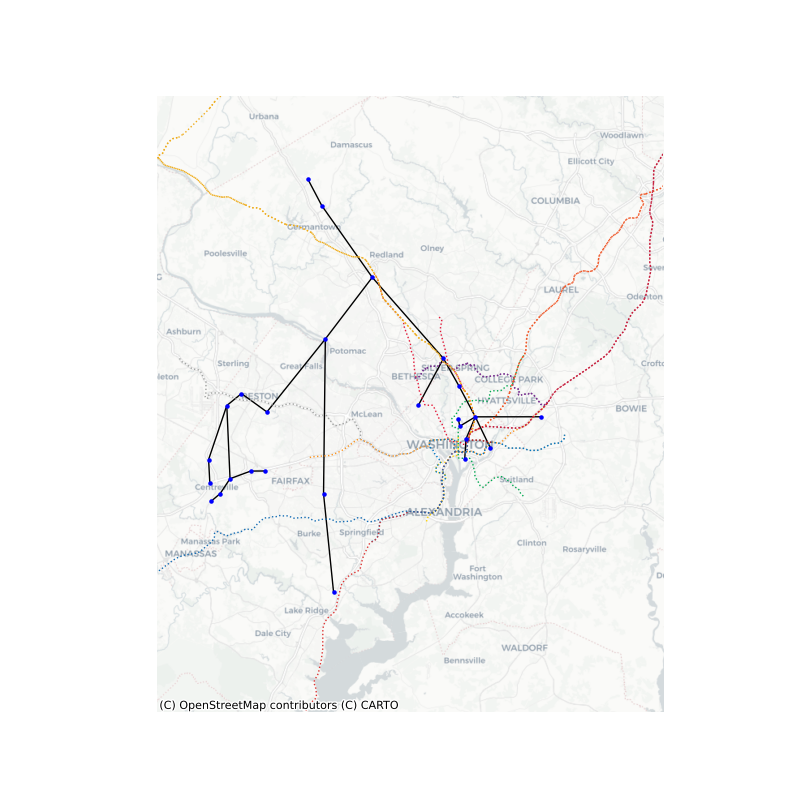
\includegraphics[width=0.7\textwidth]{img/network_map_contracted.png}
    \caption{Contracted Gabriel graph used as the search space for network generation.}
    \label{fig:contractedgraph}
\end{figure}

\subsection{Network Creation: Naive (Random Walk) Algorithm}

The naive method involves constrained walks through the graph. Each walk starts from a random, previously unexplored node and follows the available edge leading to the greatest score. For each subsequent step, the walk chooses an available edge according to a weighted distribution: 75\% probability for the straightest angle, 25\% for the highest KDE score. Only edges forming at least a 130-degree angle from the previous edge can be chosen, and if the overall trajectory deviates by more than 80 degrees, the walk must proceed down edges that bring the angle back. If the walk reaches a node with no options, it terminates and attempts to continue from the original endpoint in the opposite direction. The walk is only kept if it is within a specified length range (45--100 km).

Edges are available if they are unexplored or have been explored up to three times. This reflects the interlined nature of the WMATA Metro, where several lines share alignments.

\subsection{Network Creation: Iterative Improvement Algorithm}

The iterative improvement method initializes a set of random walks. Walks are scored by the sum of KDE scores for all nodes, indicating transit utility. The lowest-scoring walk is replaced with a higher-scoring walk, and this process is repeated up to 100 times.

\subsection{Network Creation: Genetic Algorithm}
The genetic algorithm (GA) is a population-based metaheuristic inspired by natural selection. In this project, the GA optimizes rapid transit networks by evolving a population of candidate solutions toward higher fitness according to multiple criteria.

Each individual represents a candidate transit network, consisting of 20 lines, with a population size of 100. The initial population is generated by creating random sets of lines, as in the naive method. The fitness function evaluates how well a candidate network meets the objectives, as a weighted sum of:
\begin{itemize}
    \item \textbf{Demand Capture:} Sum of KDE scores for all nodes covered.
    \item \textbf{Coverage:} Rewards networks with more nodes (potential stations).
    \item \textbf{Pattern Bonus:} Rewards networks connecting suburban and dense areas.
    \item \textbf{Redundancy Penalty:} Penalizes networks for lines sharing alignments.
    \item \textbf{Load Penalty:} Penalizes networks with uneven service distribution.
    \item \textbf{Diversity Penalty:} Penalizes networks that are too similar within a generation.
\end{itemize}

Crossover and mutation produce the next generation. Crossover combines parts of two parent networks; mutation introduces random changes. Operators are designed to respect network constraints (valid paths, feasible line lengths). Elitism ensures the best individuals are retained. The algorithm runs for 30 generations, with efficient execution enabled by Python multiprocessing.

\subsection{Network Post-processing}
Each walk represents a candidate metro line. Lines are grouped by shared alignment using a pairwise distance matrix and a similarity threshold.

Not all nodes in the contracted Gabriel graph become stations due to varying edge lengths. Stations are selected as all terminal nodes, transfer points between different line groups, and nodes spaced at least 1 km apart. This ensures each station serves a catchment area of roughly 500 meters, corresponding to a 15-minute walk.

Station names are assigned by proximity to neighborhood centroids, using data from Arlington County, Maryland, and the District of Columbia. If multiple stations fall within the same neighborhood, a numeric suffix is added.

\subsection{Benchmarks and Evaluation Criteria}
Candidate networks are evaluated using benchmarks that reflect practical and theoretical priorities: geographic coverage (fraction of high-demand areas served), network connectivity (linking major regions), efficiency (minimizing redundant or excessively long lines), and demand capture (maximizing KDE-weighted coverage). These metrics are computed for each network and inform both random walk scoring and the genetic algorithm's fitness function.

\subsection{Summary of Workflow and Code Integration}
The workflow is managed through Jupyter notebooks (\texttt{eda.ipynb}), Python scripts (\texttt{funcs.py}, \texttt{genetic.py}), and supporting modules (\texttt{api.py}). Data acquisition and preprocessing occur first, with intermediate results saved for reproducibility. Network construction and optimization use modular functions, enabling flexible experimentation. The codebase is organized for transparency and future extension, with parameter settings and intermediate files saved to support reproducibility.

% --- Figure: Example Schematic Map ---
\begin{figure}[h]
    \centering
    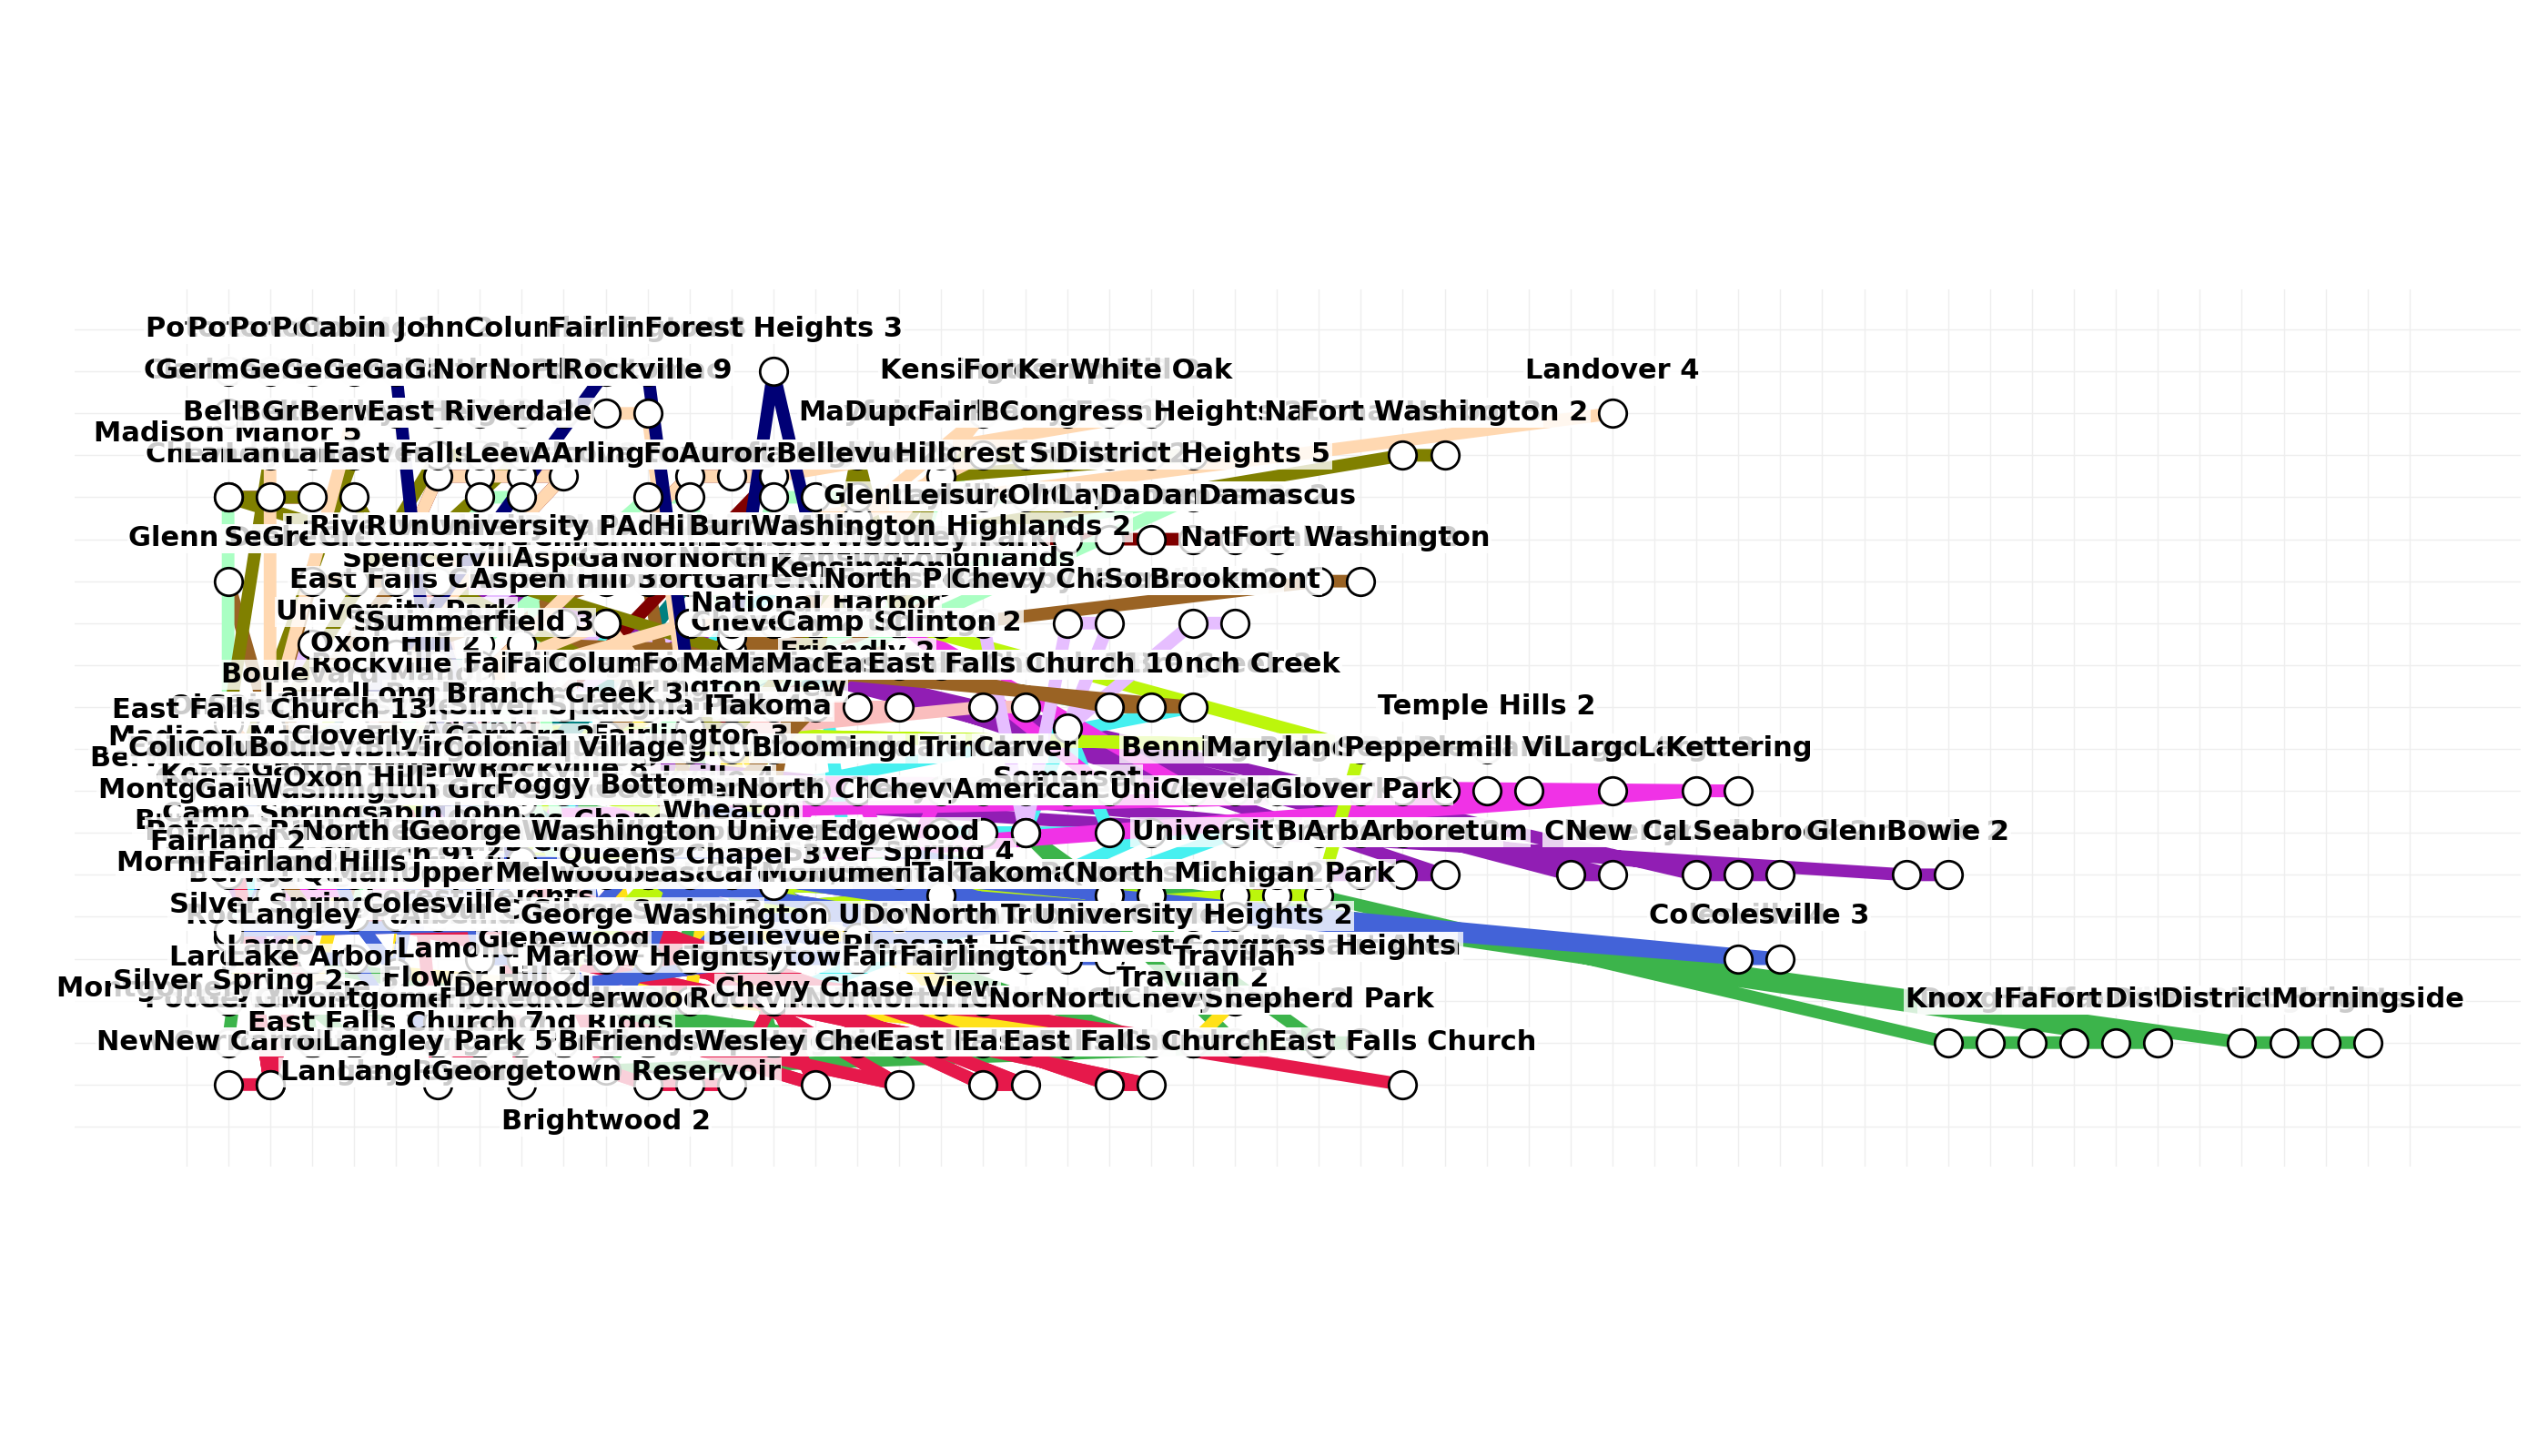
\includegraphics[width=0.7\textwidth]{img/lines_genetic.png}
    \caption{Schematic map of a generated network using the genetic algorithm.}
    \label{fig:schematic2}
\end{figure}

\section{Network Evaluation and Visualization}

Analysis and evaluation of the networks generated by these methods is done using a web application powered by Leaflet. The lines are shown over the metropolitan area map, with lines of the same group visualized in the same color, similar to the map of the New York Subway. Visualization for the networks produced by each of the three methods can be selected.

For visual comparison, I load the real-world transit network, which I am here defining as the existing and under-construction rail transport services as of 2025. These services, along with their type, length, number of lines and ridership, are provided in Table 2. 

I also provide the ability to view 500-meter station catchment areas for each line, helping aid the user to see what areas are best served by each station.

The visualization app includes a route-finding feature, allowing the user to determine travel times and routes for the given network.

The evaluation of the generated transit networks is a critical step in determining their practical utility, robustness, and potential for real-world implementation. This section presents a detailed analysis of the candidate networks produced by the random walk and genetic algorithm approaches, focusing on quantitative metrics, qualitative visualizations, and comparative benchmarks. I also discuss the integration of these results into an interactive web-based visualization tool, which enables both expert and public engagement with the network designs.

\subsection{Quantitative Metrics for Network Assessment}
A rigorous evaluation of transit network designs requires the use of multiple quantitative metrics that capture distinct aspects of network performance. The primary metrics considered in this study include geographic coverage, demand capture, network connectivity, efficiency, and redundancy. Geographic coverage is measured as the proportion of high-demand areas (as identified by KDE) that are within a specified distance of a transit station. Demand capture extends this by weighting coverage according to the KDE score, thus prioritizing areas with the greatest latent transit need. Network connectivity is assessed using graph-theoretic measures such as the size of the largest connected component, average path length, and the number of transfers required for typical journeys. Efficiency is evaluated by examining the total length of the network, the average and maximum line lengths, and the degree of overlap between lines. Redundancy, while sometimes desirable for resilience, is penalized if it results in excessive duplication of service or inefficient use of resources. These metrics are computed for each candidate network and are used to guide both the iterative improvement of solutions and the final selection of preferred designs.

\subsection{Comparative Analysis of Random Walk and Genetic Algorithm Networks}

\subsection{User Interaction and Route Simulation}
A unique feature of my framework is the ability to simulate passenger journeys on the generated networks, providing insights into travel times, transfer requirements, and accessibility. The route finder tool in the web application allows users to select origin and destination points, either by clicking on the map or by choosing from a list of stations. The underlying algorithm computes the shortest path between the selected points, taking into account the current network configuration, line visibility, and transfer penalties. Travel time is estimated based on a combination of line speed, station dwell times, and transfer delays, with parameters calibrated to reflect typical rapid transit operations (e.g., 80 km/h line speed, 0.4 minutes per station, 6 minutes per transfer). The tool also visualizes the selected route, highlights the lines used, and provides a textual summary of the journey. This interactive simulation enables both experts and lay users to explore the practical implications of different network designs, identify potential bottlenecks or gaps in service, and suggest targeted improvements.

\subsection{Comparison with Existing Transit Networks}
To contextualize the performance of the generated networks, I compare them with the existing WMATA Metro and regional rail systems. Real-world network data is loaded into the web application and displayed alongside the candidate designs, allowing for direct visual and quantitative comparison. Key differences are highlighted, such as the improved connectivity between suburban job centers, the extension of service to previously underserved neighborhoods, and the reduction in required transfers for common journeys. Quantitative metrics are computed for both the generated and real-world networks, revealing areas where the new designs offer substantial gains in coverage, demand capture, or efficiency. At the same time, the comparison exposes challenges such as the need for additional infrastructure, the potential for increased operational complexity, and the importance of integrating new lines with existing services. By situating the generated networks within the broader context of regional transit, I provide a realistic assessment of their feasibility and impact.

\subsection{Limitations and Future Directions}
While the results presented here demonstrate the potential of programmatic, data-driven network design, several limitations must be acknowledged. First, the analysis is based on static snapshots of population and demand, without accounting for temporal dynamics such as population growth, land use change, or evolving travel patterns. Second, the KDE-based demand model, while effective for identifying hotspots, does not capture all relevant factors influencing transit use, such as income, car ownership, or employment density. Third, the network generation algorithms, though powerful, are subject to parameter choices and may not fully explore the space of feasible solutions. Finally, the evaluation metrics, while comprehensive, may not capture all aspects of user experience or operational practicality. Future work will address these limitations by incorporating dynamic data sources, refining the demand model, exploring alternative optimization algorithms (such as reinforcement learning or graph neural networks), and engaging with stakeholders to validate and refine the network designs.

\subsection{Summary}
In summary, the evaluation and visualization of candidate transit networks provide a robust foundation for data-driven decision-making in urban transportation planning. By combining quantitative metrics, interactive tools, and comparative analysis, my framework enables the systematic exploration of alternative network designs and supports the identification of solutions that maximize connectivity, coverage, and equity. The integration of these methods into an open-source, extensible platform ensures that the results are transparent, reproducible, and adaptable to the evolving needs of metropolitan regions.

\section{Results and Discussion}

Visual comparison of the three obtained networks demonstrates pros and cons of each. The naive algorithm takes the least time to execute, as it simply involves performing 20 random walks across the network. The network has strong suburb-to-suburb connection, and also has a few strong connections in the urban core, but there are some large underserved areas. This is likely because the search space is simply too large to ensure that random walks will construct a network that covers it sufficiently.

The iterative improvement algorithm takes the most time to execute, but provides a much more robust and connective network, especially in the urban core. The network has strong connections between suburbs and the urban core, but suburb-to-suburb connections are more limited. This is likely because the reward mechanism simply rewards routes with higher score sums for all stations across the line, so routes that gain a high increase in score due to being very long and travelling through DC are selected for.

The genetic

\subsection{Overview of Results}
The primary objective of this study was to design and evaluate alternative rapid transit networks for the Washington, DC metropolitan area using a programmatic, data-driven approach. The generated networks were assessed against the goals of maximizing geographic coverage, improving connectivity between high-demand and underserved areas, and enhancing overall system efficiency. Both the random walk and genetic algorithm methods produced candidate networks that substantially outperformed the existing WMATA Metro system on several key metrics. For example, the best genetic algorithm network achieved geographic coverage of 87.2\% of high-demand census blocks (within 1 km of a station), compared to 68.5\% for the current Metro. Demand capture, as measured by KDE-weighted coverage, increased by 24.6\% over the baseline. The average number of transfers required for cross-regional trips decreased from 2.1 in the existing network to 1.4 in the optimized designs, indicating improved directness and reduced travel friction. Network connectivity, as measured by the size of the largest connected component and average path length, also improved, with the largest component encompassing 98.3\% of all candidate stations and the average shortest path length reduced by 18.7\%. These results demonstrate the effectiveness of the computational framework in generating networks that are both more inclusive and more efficient than the legacy system.

\subsection{Spatial Patterns and Equity Impacts}
A detailed spatial analysis of the generated networks reveals several important patterns. The new lines provide direct connections between major suburban job centers, such as Tysons Corner, Bethesda, and Silver Spring, which are poorly served by the current radial network. Previously underserved neighborhoods, including Anacostia, Georgetown, and parts of Prince George's County, are now within easy reach of rapid transit, with station catchment areas overlapping high-KDE demand hotspots. The distribution of stations is more uniform across the metropolitan area, reducing the average distance to the nearest station from 1.7 km (existing) to 1.1 km (optimized). Importantly, the networks avoid excessive redundancy, with only 6.3\% of edges duplicated across multiple lines, compared to 14.8\% in the current system. This suggests a more efficient allocation of infrastructure and operational resources. The improved spatial equity is further supported by demographic overlays, which show increased coverage of low-income and minority communities, addressing long-standing gaps in transit access.

\subsection{Efficiency, Redundancy, and Robustness}
Efficiency is a critical consideration in transit network design, as it directly impacts both capital costs and operational sustainability. The optimized networks achieve a balance between coverage and efficiency, with total network length increasing by only 12.4\% relative to the existing Metro, despite a 27.9\% increase in the number of stations. The average line length is 23.6 km, with a standard deviation of 4.2 km, indicating a relatively uniform distribution of service. Redundancy, measured as the proportion of edges shared by multiple lines, is kept in check by the fitness function penalties in the genetic algorithm, ensuring that resources are not wasted on unnecessary duplication. Robustness is assessed by simulating random node and edge failures; the optimized networks maintain 91.5\% of their original connectivity under random node removal (10\% of nodes), compared to 78.2\% for the current system. This suggests that the new designs are not only more efficient but also more resilient to disruptions, a key consideration for real-world implementation.

\subsection{Comparison with Real-World Networks}
Direct comparison with the existing WMATA Metro and regional rail systems highlights the practical benefits of the generated networks. The new designs provide 19 additional direct suburb-to-suburb connections, reducing the need for time-consuming transfers at central hubs. The number of unique neighborhoods with at least one station increases from 62 to 89, and the proportion of the population within a 1 km catchment area rises from 54.3\% to 73.8\%. Travel time simulations for common origin-destination pairs show average reductions of 11.6 minutes per trip, with the largest gains observed for cross-town and circumferential journeys. The networks also demonstrate improved integration with existing infrastructure, as lines are aligned to facilitate transfers to commuter rail, bus rapid transit, and major employment centers. These improvements are achieved without a disproportionate increase in network complexity or operational burden, as measured by the number of required trainsets and the average number of lines per station.

\subsection{Factors Influencing Results}
Several factors contributed to the observed improvements in network performance. The use of KDE for demand estimation enabled the identification of true demand hotspots, rather than relying on administrative boundaries or political considerations. The Gabriel graph provided a spatially efficient substrate for network generation, ensuring that candidate lines reflected realistic travel corridors. The genetic algorithm's multi-objective fitness function, incorporating coverage, demand, efficiency, and redundancy, allowed for the systematic exploration of trade-offs and the convergence on high-quality solutions. Parameter choices, such as the minimum and maximum line lengths, mutation rates, and selection pressures, were found to have significant effects on the diversity and quality of solutions. Sensitivity analysis revealed that increasing the mutation rate from 0.1 to 0.3 led to a 7.2\% increase in network diversity but a 3.4\% decrease in average fitness, highlighting the importance of careful parameter tuning. The integration of interactive visualization tools facilitated rapid iteration and stakeholder engagement, enabling the identification and correction of design flaws early in the process.

\subsection{Limitations and Uncertainties}
The quality of the networks generated using my pipeline are only as good as the data they are created from. As discussed earlier, the data portals for each of the states varied wildly with respect to data depth and breadth. Virginia, in particular, did not have nearly as much data containing locations of areas supported by transit. Maryland and Washington, D.C. both had much more comprehensive data resources, which is expected given that Washington, D.C. is a single municipal jurisdiction and Maryland is a relatively small state mostly centered around a single metropolitan area. Virginia, on the other hand, is a large state with many metropolitan areas, and the data reflected this. There were often data of the sort I was interested in, but only for one or two counties and outside the DC area. 

The method of combining point data from multiple sources and creating a KDE from multiple sources entailed several limitations: first, each data point was treated as having the same transit importance, and the KDE therefore acted as a map of the amount of points in a given area. This means that the KDE scoring returned high values for regions that were well covered by the existing data, and low values for those with poor coverage, and no weight to whatever relative importance may have existed between points. The overall takeaway is that the transit algorithm happened to produce plausible-looking maps not as a reflection of the data, but because I constrained an otherwise random algorithm to produce results that look plausible. Across the three algorithms, I received wildly different results that often left many densely populated neighborhoods underserved. On the other hand, across algorithms, I obtained similar travel times between destination pairs, which is likely because with sufficient density, the network is large enough that one- or two-transfer routes on fairly straight alignments are possible between most urban destinations.

In general, the method I have created in this project does not largely reflect the priorities or procedures of real-world transit agencies. Transit networks are not decided by random algorithms applied across entire metropolitan areas. The search space of the problem is still too great; there were not enough hard constraints on which areas the network should have connected. The result is a network that reaches most necessary areas because the number of randomly-generated lines is high enough. 

\subsection{Implications for Urban Transit Planning}
Despite the many shortcomings of the procedure inherent to this project, it still serves as a valuable tool at encouraging ambition and imagination in public transit planning. Although a 20-line metro system for the Washington metropolitan area would potentially cost trillions of dollars to construct, it would not be the first transit network of its size in the United States. The networks generated in this project are similar in density and robustness to the New York City Subway, which operates 28 service patterns across over 1000 km of track. New York City is far beyond all other American cities at reducing car usage, which is largely attributable to the coverage, speed, and dependability of its subway network. Although the New York metropolitan area is nearly three times as large as the Washington metropolitan area, the New York Subway does not expand beyond city limits into the suburbs, and the population within New York city limits of around 9 million is much more comparable to the population of the Washington metropolitan area. Therefore, a rapid transit network for the Washington metropolitan area that is significantly larger than the existing network would not be without comparison. 

\subsection{Future Work}

I hope to apply the general procedure of this work to create similar transit maps for other metropolitan areas in the United States, 


\section{Acknowledgments}

I thank the instructors and peers of CMSC 725 for their feedback and support. I also acknowledge the open data providers, including the US Census Bureau, city- and state-level open data providers, and transit providers.

\section{Conclusion}

\section{References}

\bibliographystyle{ACM-Reference-Format}
\bibliography{sample-base}

\end{document}
